\section{Droplet Formation Simulation}

To provide an educational yet illustrative understanding of droplet ejection,
a simplified capillary–inertial nozzle model was implemented.
The model uses lumped parameters (nozzle radius, viscosity, surface tension,
density, and trapezoidal drive pulses) to approximate meniscus velocity
and ejected volume.

\begin{figure}[htbp]
  \centering
  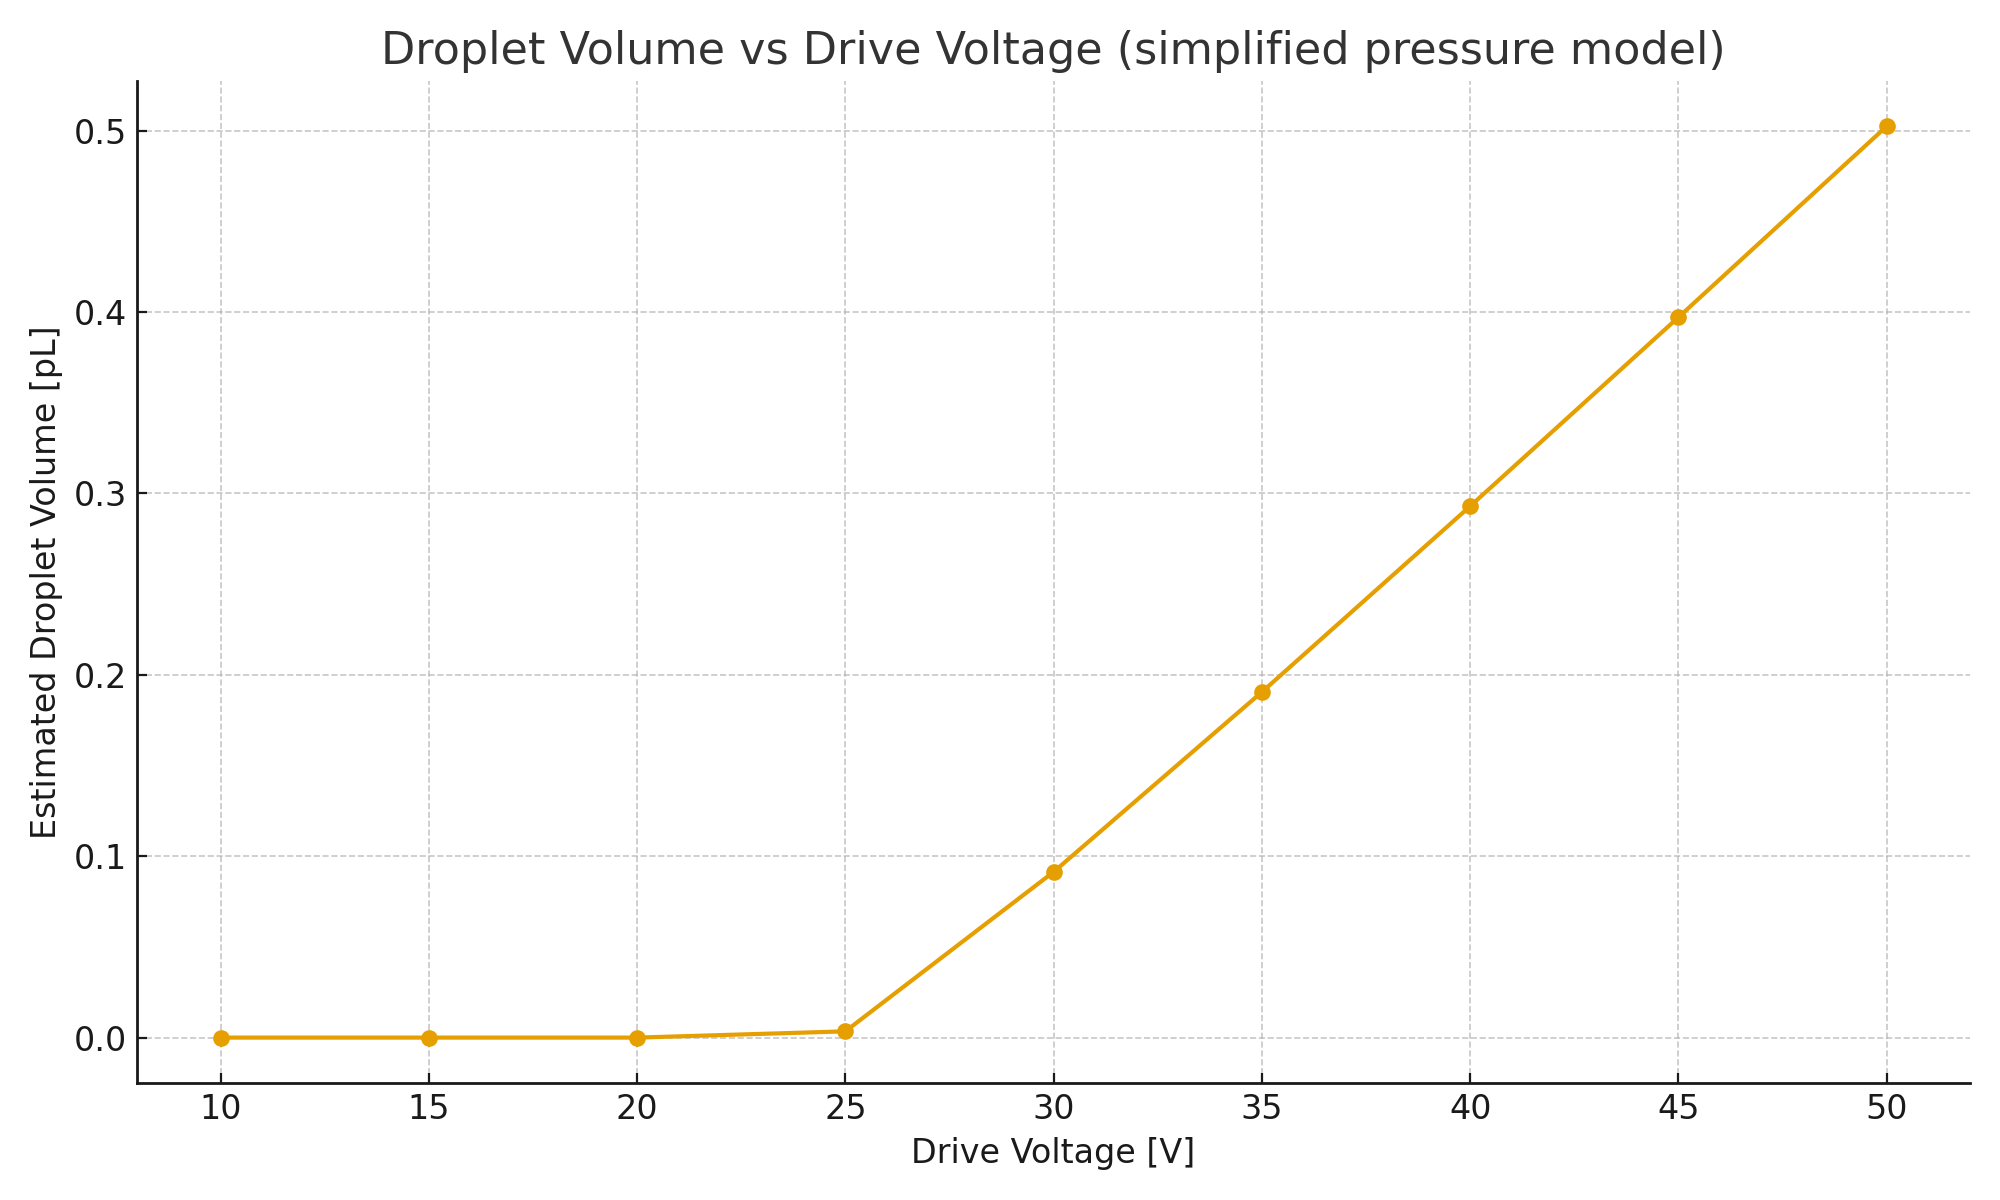
\includegraphics[width=0.9\linewidth]{figs/droplet_volume_vs_voltage.png}
  \caption{Estimated droplet volume versus drive voltage
  using the simplified lumped model (5--50~V).}
  \label{fig:voltage_vs_volume}
\end{figure}

Representative time traces at 10, 30, and 50~V show the meniscus velocity
profiles (Fig.~\ref{fig:vel_traces}).

\begin{figure}[htbp]
  \centering
  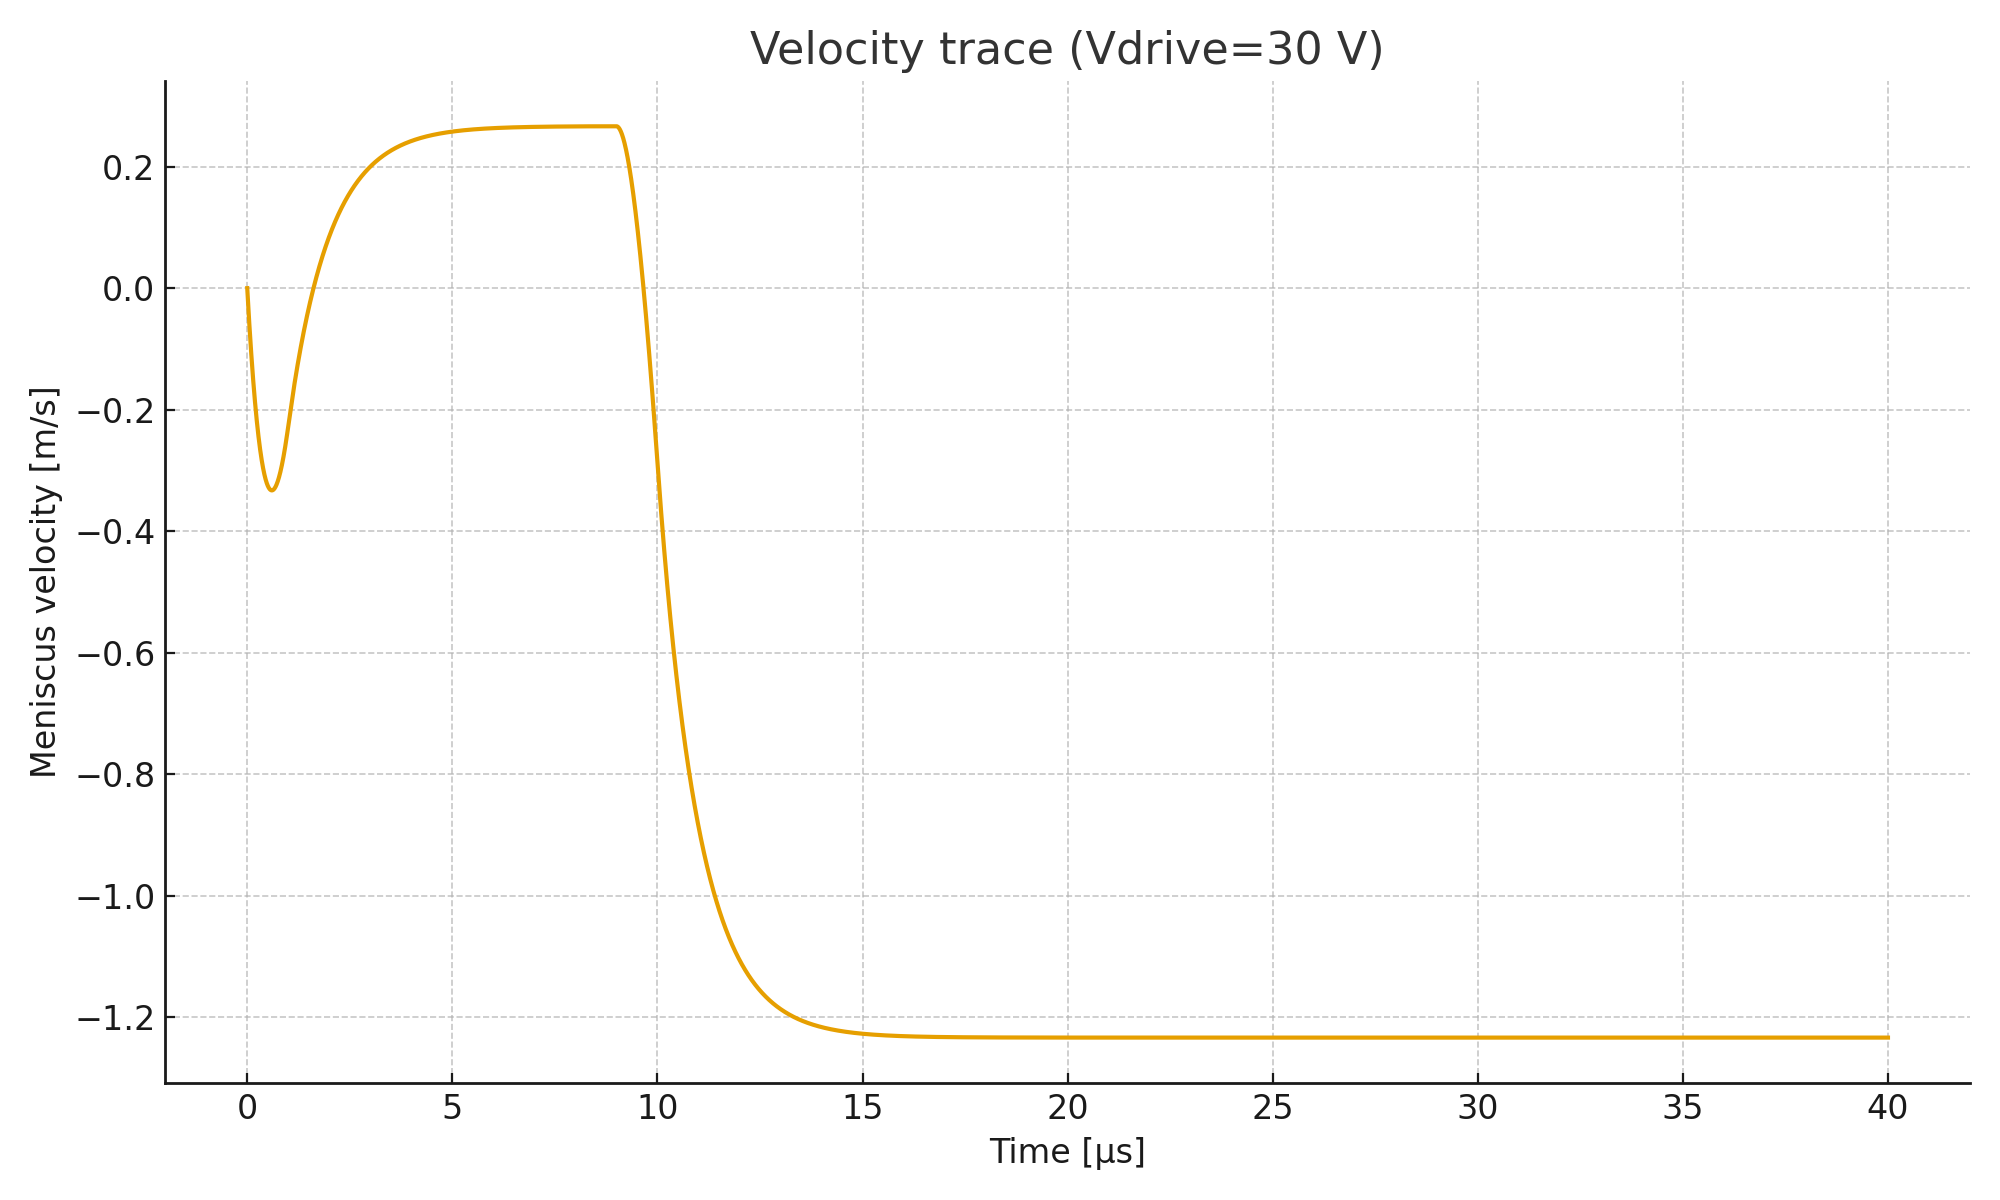
\includegraphics[width=0.9\linewidth]{figs/velocity_trace_30V.png}
  \caption{Example meniscus velocity trace for 30~V drive pulse.}
  \label{fig:vel_traces}
\end{figure}
